%********************************************************************
% Appendix
%*******************************************************


\chapter{Appendix}

\renewcommand{\thechapter}{A}

%----------------------------------------------------------------------------------------


%----------------------------------------------------------------------------------------

\subsection*{Photo of the Simulated Underwater Robot}

\vspace{-0.4cm}

\begin{figure}[h]
	\centering	
	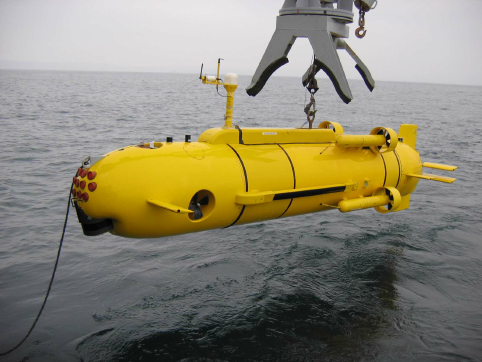
\includegraphics[width=\textwidth]{Figures/redermor.png}			
	\caption[The autonomous underwater vehicle \emph{Redermor} developed by GESMA.]{The autonomous underwater vehicle \emph{Redermor}, developed by GESMA (Groupe d'Etude Sous-Marine de l'Atlantique).}		
	\label{fig:redermor}			
\end{figure}



\subsection*{Additional Results in Scenario 1 with 2 Landmarks}

Table \ref{tab:results_scenario1} and \ref{tab:results_scenario1_kidnapping} list the figures depicting the estimation results for Scenario 1, with and without kidnapping, respectively.

\subsection*{Additional Results in Scenario 2 with 4 Landmarks}

Table \ref{tab:results_scenario2} and \ref{tab:results_scenario2_kidnapping} list the figures depicting the estimation results for Scenario 2, with and without kidnapping, respectively.

\subsection*{Additional Results in Scenario 3 with 9 Landmarks}

Table \ref{tab:results_scenario3} and \ref{tab:results_scenario3_kidnapping} list the figures depicting the estimation results for Scenario 3, with and without kidnapping, respectively.

\begin{table*}
\centering
\ra{1.3}\begin{tabular}{@{}llrrrr@{}}
\toprule
\thead{\normalsize Box \\ \normalsize plots} & \thead{\normalsize Mean \\ \normalsize errors} & \phantom{a} & \multicolumn{3}{c}{Number of particles} \\
\midrule
& & & \texttt{PF} / \texttt{PFC} / \texttt{PFS} & \phantom{a} & \texttt{UPF} / \texttt{UPFC} / \texttt{UPFS} \\
\cmidrule{4-4} \cmidrule{6-6}
\ref{fig:2018-09-30-12-09-00-results-figure-1} & \ref{fig:2018-09-30-12-09-00-results-figure-5}, \ref{fig:2018-09-30-12-09-00-results-figure-7} & & 10000 & & 1000 \\ 
\ref{fig:2018-09-29-14-05-04-results-figure-1} & \ref{fig:2018-09-29-14-05-04-results-figure-5}, \ref{fig:2018-09-29-14-05-04-results-figure-7} & & 1000 & & 100 \\
%\ref{fig:2018-09-28-14-27-04-results-figure-1} & \ref{fig:2018-09-28-14-27-04-results-figure-5}, \ref{fig:2018-09-28-14-27-04-results-figure-7} & & 100 & & 10 \\ 
\bottomrule
\end{tabular}
\caption{List of figures depicting the estimation results in Scenario 1.}
\label{tab:results_scenario1}
\end{table*}


\begin{table*}
\centering
\ra{1.3}\begin{tabular}{@{}llrrrr@{}}
\toprule
\thead{\normalsize Box \\ \normalsize plots} & \thead{\normalsize Mean \\ \normalsize errors} & \phantom{a} & \multicolumn{3}{c}{Number of particles} \\
\midrule
& & & \texttt{PF} / \texttt{PFC} / \texttt{PFS} & \phantom{a} & \texttt{UPF} / \texttt{UPFC} / \texttt{UPFS} \\
\cmidrule{4-4} \cmidrule{6-6}
\ref{fig:2018-10-04-15-13-55-results-figure-1} & \ref{fig:2018-10-04-15-13-55-results-figure-6}, \ref{fig:2018-10-04-15-13-55-results-figure-8} & & 10000 & & 1000 \\ 
\ref{fig:2018-09-30-01-28-57-results-figure-1} & \ref{fig:2018-09-30-01-28-57-results-figure-6}, \ref{fig:2018-09-30-01-28-57-results-figure-8} & & 1000 & & 100 \\ 
%\ref{fig:2018-09-28-21-07-55-results-figure-1} & \ref{fig:2018-09-28-21-07-55-results-figure-6}, \ref{fig:2018-09-28-21-07-55-results-figure-8} & & 100 & & 10 \\ 
\bottomrule
\end{tabular}
\caption{List of figures depicting the estimation results in Scenario 1 with kidnapping.}
\label{tab:results_scenario1_kidnapping}
\end{table*}




\begin{table*}
\centering
\ra{1.3}\begin{tabular}{@{}llrrrr@{}}
\toprule
\thead{\normalsize Box \\ \normalsize plots} & \thead{\normalsize Mean \\ \normalsize errors} & \phantom{a} & \multicolumn{3}{c}{Number of particles} \\
\midrule
& & & \texttt{PF} / \texttt{PFC} / \texttt{PFS} & \phantom{a} & \texttt{UPF} / \texttt{UPFC} / \texttt{UPFS} \\
\cmidrule{4-4} \cmidrule{6-6}
\ref{fig:2018-09-24-11-26-33-results-figure-1} & \ref{fig:2018-09-24-11-26-33-results-figure-5}, \ref{fig:2018-09-24-11-26-33-results-figure-7} & & 10000 & & 100 \\ 
\ref{fig:2018-09-23-20-54-13-results-figure-1} & \ref{fig:2018-09-23-20-54-13-results-figure-5}, \ref{fig:2018-09-23-20-54-13-results-figure-7} & & 1000 & & 10 \\ 
%\ref{fig:2018-09-21-16-00-07-results-figure-1} & \ref{fig:2018-09-21-16-00-07-results-figure-5}, \ref{fig:2018-09-21-16-00-07-results-figure-7} & & 100 & & 10 \\ 
\bottomrule
\end{tabular}
\caption{List of figures depicting the estimation results in Scenario 2.}
\label{tab:results_scenario2}
\end{table*}


\begin{table*}
\centering
\ra{1.3}\begin{tabular}{@{}llrrrr@{}}
\toprule
\thead{\normalsize Box \\ \normalsize plots} & \thead{\normalsize Mean \\ \normalsize errors} & \phantom{a} & \multicolumn{3}{c}{Number of particles} \\
\midrule
& & & \texttt{PF} / \texttt{PFC} / \texttt{PFS} & \phantom{a} & \texttt{UPF} / \texttt{UPFC} / \texttt{UPFS} \\
\cmidrule{4-4} \cmidrule{6-6}
\ref{fig:2018-09-21-21-56-07-results-figure-1} & \ref{fig:2018-09-21-21-56-07-results-figure-6}, \ref{fig:2018-09-21-21-56-07-results-figure-8} & & 10000 & & 100 \\ 
\ref{fig:2018-09-23-12-42-11-results-figure-1}& \ref{fig:2018-09-23-12-42-11-results-figure-6}, \ref{fig:2018-09-23-12-42-11-results-figure-8} & & 1000 & & 10 \\ 
%\ref{fig:2018-09-21-10-11-38-results-figure-1}& \ref{fig:2018-09-21-10-11-38-results-figure-6}, \ref{fig:2018-09-21-10-11-38-results-figure-8} & & 100 & & 10 \\ 
\bottomrule
\end{tabular}
\caption{List of figures depicting the estimation results in Scenario 2 with kidnapping.}
\label{tab:results_scenario2_kidnapping}
\end{table*}

\clearpage


\begin{table*}[h!]
\centering
\ra{1.3}\begin{tabular}{@{}llrrrr@{}}
\toprule
\thead{\normalsize Box \\ \normalsize plots} & \thead{\normalsize Mean \\ \normalsize errors} & \phantom{a} & \multicolumn{3}{c}{Number of particles} \\
\midrule
& & & \texttt{PF} / \texttt{PFC} / \texttt{PFS} & \phantom{a} & \texttt{UPF} / \texttt{UPFC} / \texttt{UPFS} \\
\cmidrule{4-4} \cmidrule{6-6}
\ref{fig:2018-08-30-19-17-11-results-figure-1} & \ref{fig:2018-08-30-19-17-11-results-figure-4}, \ref{fig:2018-08-30-19-17-11-results-figure-6} & & 10000 & & 100 \\ 
\ref{fig:2018-09-01-16-39-24-results-figure-1} & \ref{fig:2018-09-01-16-39-24-results-figure-4}, \ref{fig:2018-09-01-16-39-24-results-figure-6} & & 1000 & & 10 \\ 
%\ref{fig:2018-09-02-11-42-39-results-figure-1} & \ref{fig:2018-09-02-11-42-39-results-figure-4}, \ref{fig:2018-09-02-11-42-39-results-figure-6} & & 100 & & 10 \\ 
\bottomrule
\end{tabular}
\caption{List of figures depicting the estimation results in Scenario 3.}
\label{tab:results_scenario3}
\end{table*}

\begin{table*}[h!]
\centering
\ra{1.3}\begin{tabular}{@{}llrrrr@{}}
\toprule
\thead{\normalsize Box \\ \normalsize plots} & \thead{\normalsize Mean \\ \normalsize errors} & \phantom{a} & \multicolumn{3}{c}{Number of particles} \\
\midrule
& & & \texttt{PF} / \texttt{PFC} / \texttt{PFS} & \phantom{a} & \texttt{UPF} / \texttt{UPFC} / \texttt{UPFS} \\
\cmidrule{4-4} \cmidrule{6-6}
\ref{fig:2018-09-03-13-54-12-results-figure-1} & \ref{fig:2018-09-03-13-54-12-results-figure-4}, \ref{fig:2018-09-03-13-54-12-results-figure-6} & & 10000 & & 100 \\ 
\ref{fig:2018-09-07-08-54-39-results-figure-1} & \ref{fig:2018-09-07-08-54-39-results-figure-4}, \ref{fig:2018-09-07-08-54-39-results-figure-6} & & 1000 & & 10 \\ 
%\ref{fig:2018-09-18-11-37-10-results-figure-1} & \ref{fig:2018-09-18-11-37-10-results-figure-5}, \ref{fig:2018-09-18-11-37-10-results-figure-7} & & 100 & & 10 \\ 
\bottomrule
\end{tabular}
\caption{List of figures depicting the estimation results in Scenario 3 with kidnapping.}
\label{tab:results_scenario3_kidnapping}
\end{table*}

%----------------------------------------------------------------------------------------


%% 2 Landmarks

% 1000 / 10

\begin{figure}
	\centering
	\setlength\figureheight{0.9\textheight} 	
	\setlength\figurewidth{1.0\textwidth}		
	\tikzsetnextfilename{2018-09-29-14-05-04-results-figure-1}		
	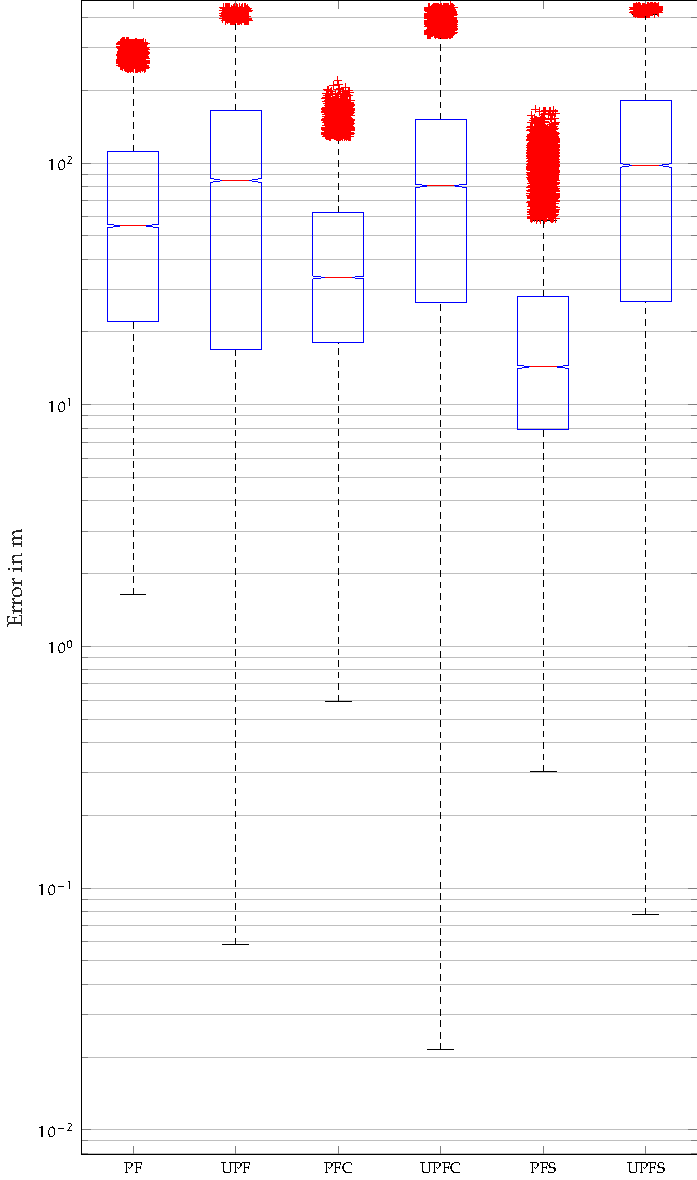
\includegraphics[width=\textwidth]{Tikz/Results/2018-09-29-14-05-04-results-figure-1.tikz}			
	\caption[Box plot of the estimation errors in Scenario 1. \texttt{PF}, \texttt{PFC}, \texttt{PFS}: 1000 particles. \texttt{UPF}, \texttt{UPFC}, \texttt{UPFS}: 100 particles.]{Box plot of the estimation errors in Scenario 1 (logarithmic scale). \texttt{PF}, \texttt{PFC}, \texttt{PFS}: 1000 particles. \texttt{UPF}, \texttt{UPFC}, \texttt{UPFS}: 100 particles.}
	\label{fig:2018-09-29-14-05-04-results-figure-1}			
\end{figure}

\begin{figure}
	\centering
	\setlength\figureheight{1.0\textwidth} 	
	\setlength\figurewidth{0.9\textheight}		
	\tikzsetnextfilename{2018-09-29-14-05-04-results-figure-5}
	\rotatebox{90}{
	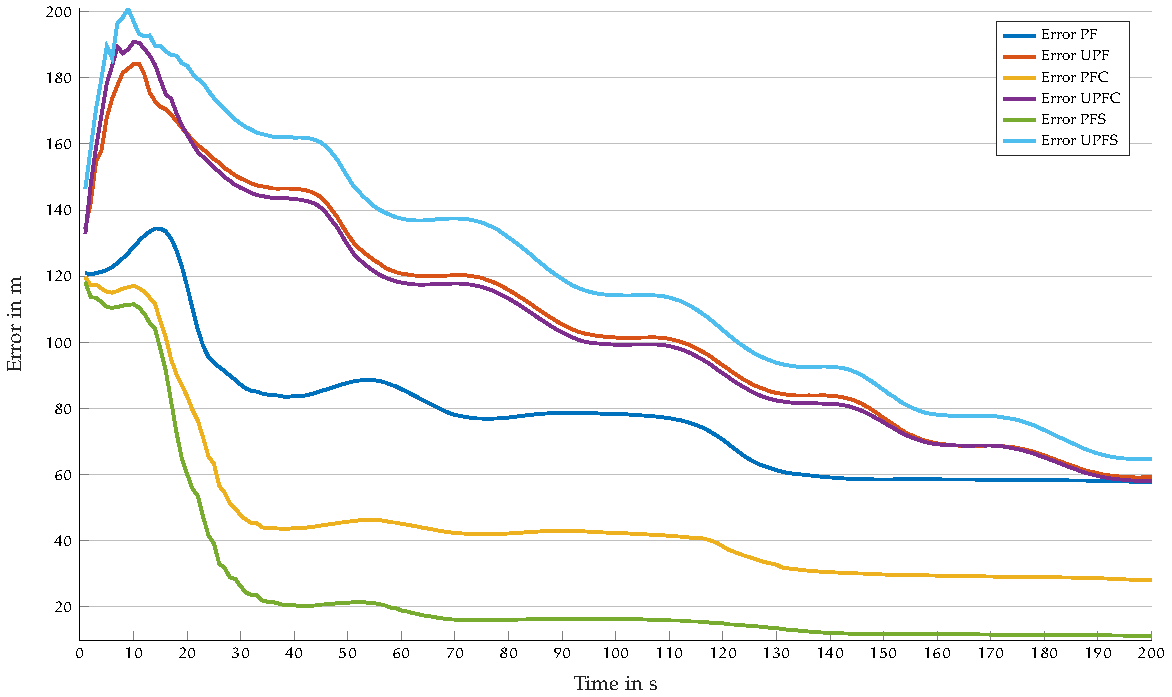
\includegraphics[height=1.0\textwidth]{Tikz/Results/2018-09-29-14-05-04-results-figure-5.tikz}}			
	\caption[Mean estimation error over time in Scenario 1. \texttt{PF}, \texttt{PFC}, \texttt{PFS}: 1000 particles. \texttt{UPF}, \texttt{UPFC}, \texttt{UPFS}: 100 particles.]{Mean estimation error over time in Scenario 1. \texttt{PF}, \texttt{PFC}, \texttt{PFS}: 1000 particles. \texttt{UPF}, \texttt{UPFC}, \texttt{UPFS}: 100 particles.}
	\label{fig:2018-09-29-14-05-04-results-figure-5}			
\end{figure}

\begin{figure}
	\centering
	\setlength\figureheight{1.0\textwidth} 	
	\setlength\figurewidth{0.9\textheight}		
	\tikzsetnextfilename{2018-09-29-14-05-04-results-figure-7}		
	\rotatebox{90}{
	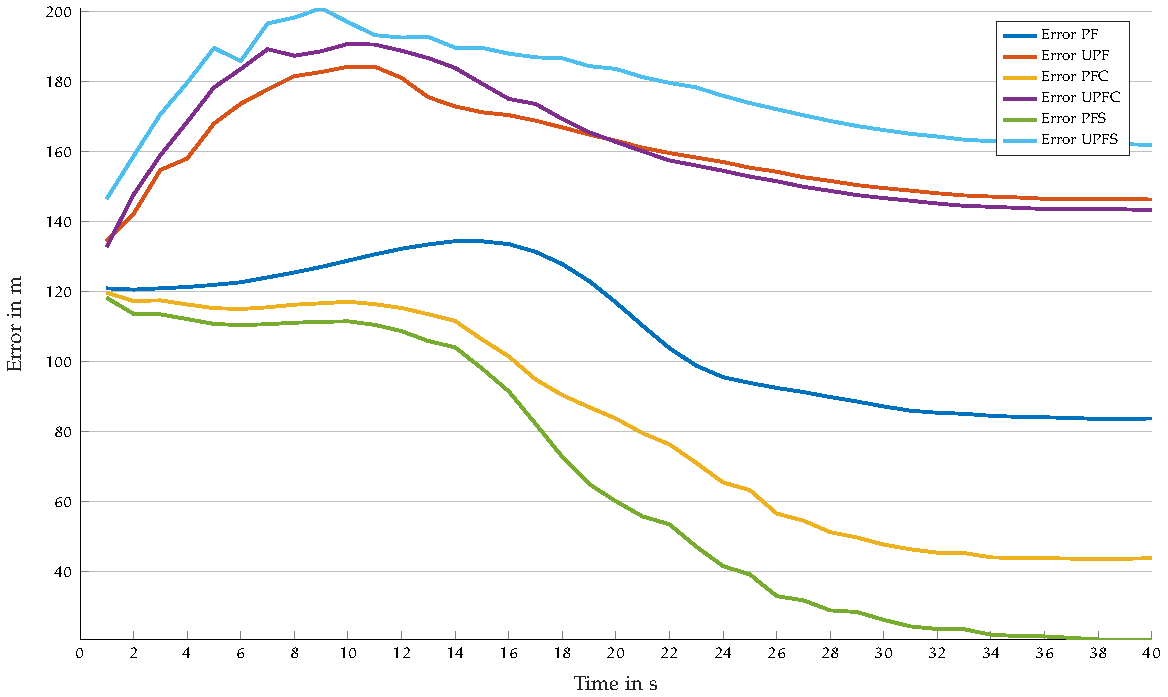
\includegraphics[height=1.0\textwidth]{Tikz/Results/2018-09-29-14-05-04-results-figure-7.tikz}}			
	\caption[First 40 seconds of the mean estimation error over time in Scenario 1. \texttt{PF}, \texttt{PFC}, \texttt{PFS}: 1000 particles. \texttt{UPF}, \texttt{UPFC}, \texttt{UPFS}: 100 particles.]{First 40 seconds of the mean estimation error over time in Scenario 1. \texttt{PF}, \texttt{PFC}, \texttt{PFS}: 1000 particles. \texttt{UPF}, \texttt{UPFC}, \texttt{UPFS}: 100 particles.}
	\label{fig:2018-09-29-14-05-04-results-figure-7}			
\end{figure}
%

% 100 / 10

%\begin{figure}
%	\centering
%	\setlength\figureheight{0.9\textheight} 	
%	\setlength\figurewidth{1.0\textwidth}		
%	\tikzsetnextfilename{2018-09-28-14-27-04-results-figure-1}		
%	\includegraphics[width=\textwidth]{Tikz/Results/2018-09-28-14-27-04-results-figure-1.tikz}			
%	\caption[Box plot of the estimation errors in Scenario 1. \texttt{PF}, \texttt{PFC}, \texttt{PFS}: 100 particles. \texttt{UPF}, \texttt{UPFC}, \texttt{UPFS}: 10 particles.]{Box plot of the estimation errors in Scenario 1 (logarithmic scale). \texttt{PF}, \texttt{PFC}, \texttt{PFS}: 100 particles. \texttt{UPF}, \texttt{UPFC}, \texttt{UPFS}: 10 particles.}
%	\label{fig:2018-09-28-14-27-04-results-figure-1}			
%\end{figure}
%
%\begin{figure}
%	\centering
%	\setlength\figureheight{1.0\textwidth} 	
%	\setlength\figurewidth{0.9\textheight}		
%	\tikzsetnextfilename{2018-09-28-14-27-04-results-figure-5}		
%	\rotatebox{90}{
%	\includegraphics[height=1.0\textwidth]{Tikz/Results/2018-09-28-14-27-04-results-figure-5.tikz}}			
%	\caption[Mean estimation error over time in Scenario 1. \texttt{PF}, \texttt{PFC}, \texttt{PFS}: 100 particles. \texttt{UPF}, \texttt{UPFC}, \texttt{UPFS}: 10 particles.]{Mean estimation error over time in Scenario 1. \texttt{PF}, \texttt{PFC}, \texttt{PFS}: 100 particles. \texttt{UPF}, \texttt{UPFC}, \texttt{UPFS}: 10 particles.}
%	\label{fig:2018-09-28-14-27-04-results-figure-5}			
%\end{figure}
%
%\begin{figure}
%	\centering
%	\setlength\figureheight{1.0\textwidth} 	
%	\setlength\figurewidth{0.9\textheight}		
%	\tikzsetnextfilename{2018-09-28-14-27-04-results-figure-7}		
%	\rotatebox{90}{
%	\includegraphics[height=1.0\textwidth]{Tikz/Results/2018-09-28-14-27-04-results-figure-7.tikz}}			
%	\caption[First 40 seconds of the mean estimation error over time in Scenario 1. \texttt{PF}, \texttt{PFC}, \texttt{PFS}: 100 particles. \texttt{UPF}, \texttt{UPFC}, \texttt{UPFS}: 10 particles.]{First 40 seconds of the mean estimation error over time in Scenario 1. \texttt{PF}, \texttt{PFC}, \texttt{PFS}: 100 particles. \texttt{UPF}, \texttt{UPFC}, \texttt{UPFS}: 10 particles.}
%	\label{fig:2018-09-28-14-27-04-results-figure-7}			
%\end{figure}

%% 2 Landmarks kidnapping

% 1000 / 100

\begin{figure}
	\centering
	\setlength\figureheight{0.9\textheight} 	
	\setlength\figurewidth{1.0\textwidth}		
	\tikzsetnextfilename{2018-09-30-01-28-57-results-figure-1}		
	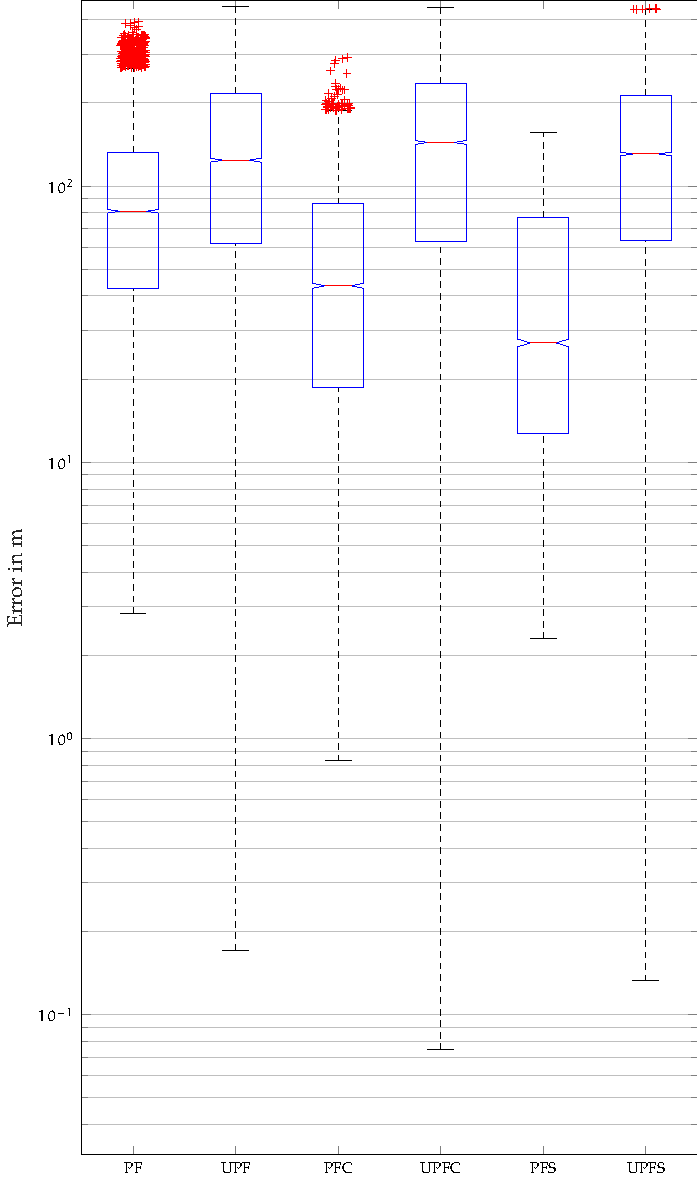
\includegraphics[width=\textwidth]{Tikz/Results/2018-09-30-01-28-57-results-figure-1.tikz}			
	\caption[Box plot of the estimation errors in Scenario 1 with kidnapping. \texttt{PF}, \texttt{PFC}, \texttt{PFS}: 1000 particles. \texttt{UPF}, \texttt{UPFC}, \texttt{UPFS}: 100 particles.]{Box plot of the estimation errors in Scenario 1 with kidnapping (logarithmic scale). \texttt{PF}, \texttt{PFC}, \texttt{PFS}: 1000 particles. \texttt{UPF}, \texttt{UPFC}, \texttt{UPFS}: 100 particles.}
	\label{fig:2018-09-30-01-28-57-results-figure-1}			
\end{figure}

\begin{figure}
	\centering
	\setlength\figureheight{1.0\textwidth} 	
	\setlength\figurewidth{0.9\textheight}		
	\tikzsetnextfilename{2018-09-30-01-28-57-results-figure-6}		
	\rotatebox{90}{
	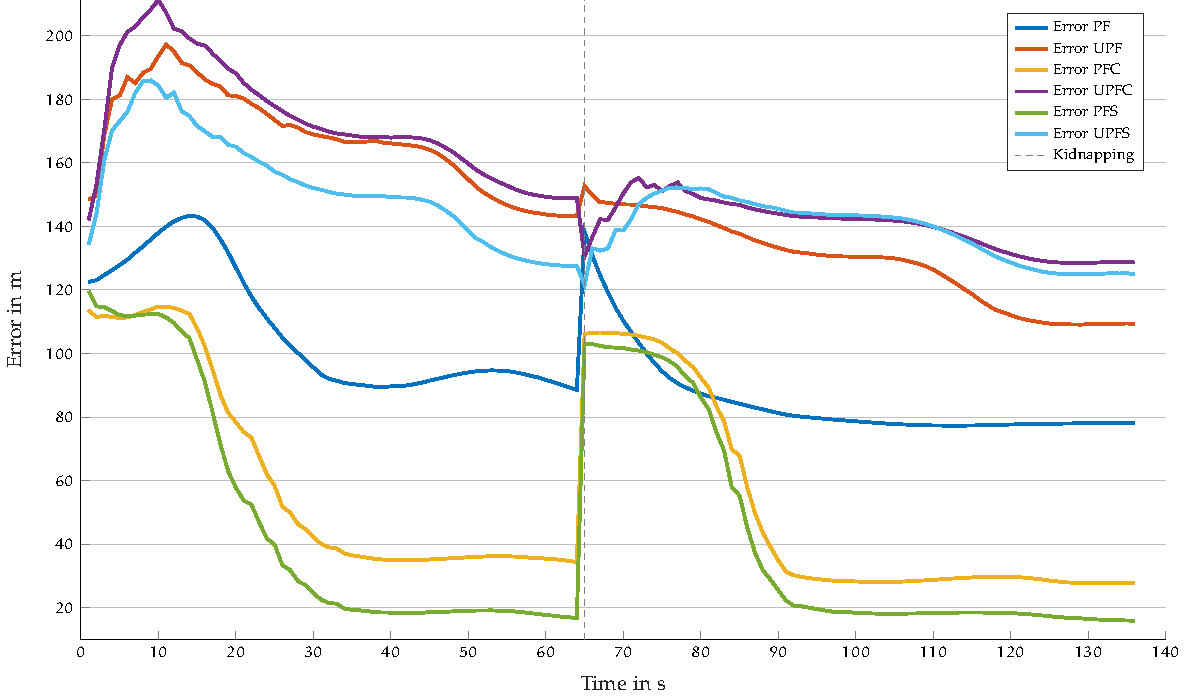
\includegraphics[height=1.0\textwidth]{Tikz/Results/2018-09-30-01-28-57-results-figure-6.tikz}}			
	\caption[Mean estimation error over time in Scenario 1 with kidnapping. \texttt{PF}, \texttt{PFC}, \texttt{PFS}: 1000 particles. \texttt{UPF}, \texttt{UPFC}, \texttt{UPFS}: 100 particles.]{Mean estimation error over time in Scenario 1 with kidnapping. \texttt{PF}, \texttt{PFC}, \texttt{PFS}: 1000 particles. \texttt{UPF}, \texttt{UPFC}, \texttt{UPFS}: 10 particles.}
	\label{fig:2018-09-30-01-28-57-results-figure-6}			
\end{figure}

\begin{figure}
	\centering
	\setlength\figureheight{1.0\textwidth} 	
	\setlength\figurewidth{0.9\textheight}		
	\tikzsetnextfilename{2018-09-30-01-28-57-results-figure-8}		
	\rotatebox{90}{
	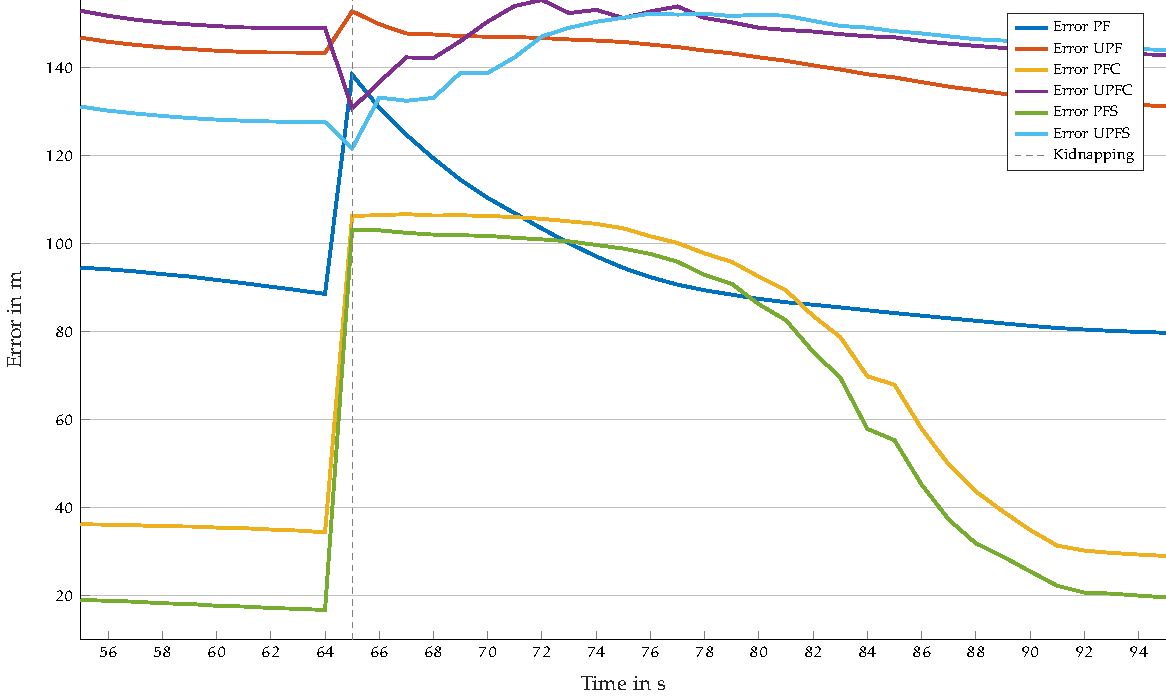
\includegraphics[height=1.0\textwidth]{Tikz/Results/2018-09-30-01-28-57-results-figure-8.tikz}}			
	\caption[First 30 seconds of the mean estimation error over time after kidnapping in Scenario 1. \texttt{PF}, \texttt{PFC}, \texttt{PFS}: 1000 particles. \texttt{UPF}, \texttt{UPFC}, \texttt{UPFS}: 10 particles.]{First 30 seconds of the mean estimation error over time after kidnapping in Scenario 1. \texttt{PF}, \texttt{PFC}, \texttt{PFS}: 1000 particles. \texttt{UPF}, \texttt{UPFC}, \texttt{UPFS}: 100 particles.}
	\label{fig:2018-09-30-01-28-57-results-figure-8}			
\end{figure}


% 100 / 10

%\begin{figure}
%	\centering
%	\setlength\figureheight{0.9\textheight} 	
%	\setlength\figurewidth{1.0\textwidth}		
%	\tikzsetnextfilename{2018-09-28-21-07-55-results-figure-1}		
%	\includegraphics[width=\textwidth]{Tikz/Results/2018-09-28-21-07-55-results-figure-1.tikz}			
%	\caption[Box plot of the estimation errors in Scenario 1 with kidnapping. \texttt{PF}, \texttt{PFC}, \texttt{PFS}: 100 particles. \texttt{UPF}, \texttt{UPFC}, \texttt{UPFS}: 10 particles.]{Box plot of the estimation errors in Scenario 1 with kidnapping (logarithmic scale). \texttt{PF}, \texttt{PFC}, \texttt{PFS}: 100 particles. \texttt{UPF}, \texttt{UPFC}, \texttt{UPFS}: 10 particles.}
%	\label{fig:2018-09-28-21-07-55-results-figure-1}			
%\end{figure}
%
%\begin{figure}
%	\centering
%	\setlength\figureheight{1.0\textwidth} 	
%	\setlength\figurewidth{0.9\textheight}		
%	\tikzsetnextfilename{2018-09-28-21-07-55-results-figure-6}		
%	\rotatebox{90}{
%	\includegraphics[height=1.0\textwidth]{Tikz/Results/2018-09-28-21-07-55-results-figure-6.tikz}}			
%	\caption[Mean estimation error over time in Scenario 1 with kidnapping. \texttt{PF}, \texttt{PFC}, \texttt{PFS}: 100 particles. \texttt{UPF}, \texttt{UPFC}, \texttt{UPFS}: 10 particles.]{Mean estimation error over time in Scenario 1 with kidnapping. \texttt{PF}, \texttt{PFC}, \texttt{PFS}: 100 particles. \texttt{UPF}, \texttt{UPFC}, \texttt{UPFS}: 10 particles.}
%	\label{fig:2018-09-28-21-07-55-results-figure-6}			
%\end{figure}
%
%\begin{figure}
%	\centering
%	\setlength\figureheight{1.0\textwidth} 	
%	\setlength\figurewidth{0.9\textheight}		
%	\tikzsetnextfilename{2018-09-28-21-07-55-results-figure-8}		
%	\rotatebox{90}{
%	\includegraphics[height=1.0\textwidth]{Tikz/Results/2018-09-28-21-07-55-results-figure-8.tikz}}			
%	\caption[First 30 seconds of the mean estimation error over time after kidnapping in Scenario 1. \texttt{PF}, \texttt{PFC}, \texttt{PFS}: 100 particles. \texttt{UPF}, \texttt{UPFC}, \texttt{UPFS}: 10 particles.]{First 30 seconds of the mean estimation error over time after kidnapping in Scenario 1. \texttt{PF}, \texttt{PFC}, \texttt{PFS}: 100 particles. \texttt{UPF}, \texttt{UPFC}, \texttt{UPFS}: 10 particles.}
%	\label{fig:2018-09-28-21-07-55-results-figure-8}			
%\end{figure}





%% 4 Landmarks


% 1000 / 10

\begin{figure}
	\centering
	\setlength\figureheight{0.9\textheight} 	
	\setlength\figurewidth{1.0\textwidth}		
	\tikzsetnextfilename{2018-09-23-20-54-13-results-figure-1}		
	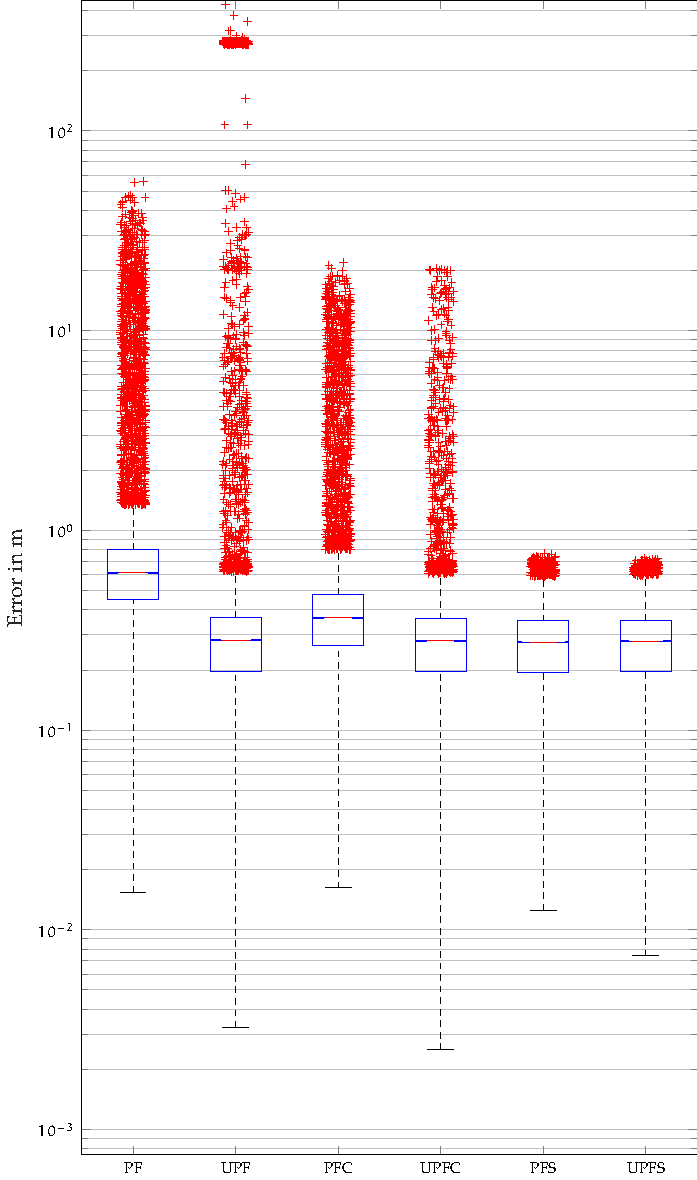
\includegraphics[width=\textwidth]{Tikz/Results/2018-09-23-20-54-13-results-figure-1.tikz}			
	\caption[Box plot of the estimation errors in Scenario 2. \texttt{PF}, \texttt{PFC}, \texttt{PFS}: 1000 particles. \texttt{UPF}, \texttt{UPFC}, \texttt{UPFS}: 10 particles.]{Box plot of the estimation errors in Scenario 2 (logarithmic scale). \texttt{PF}, \texttt{PFC}, \texttt{PFS}: 1000 particles. \texttt{UPF}, \texttt{UPFC}, \texttt{UPFS}: 10 particles.}
	\label{fig:2018-09-23-20-54-13-results-figure-1}			
\end{figure}

\begin{figure}
	\centering
	\setlength\figureheight{1.0\textwidth} 	
	\setlength\figurewidth{0.9\textheight}		
	\tikzsetnextfilename{2018-09-23-20-54-13-results-figure-5}		
	\rotatebox{90}{
	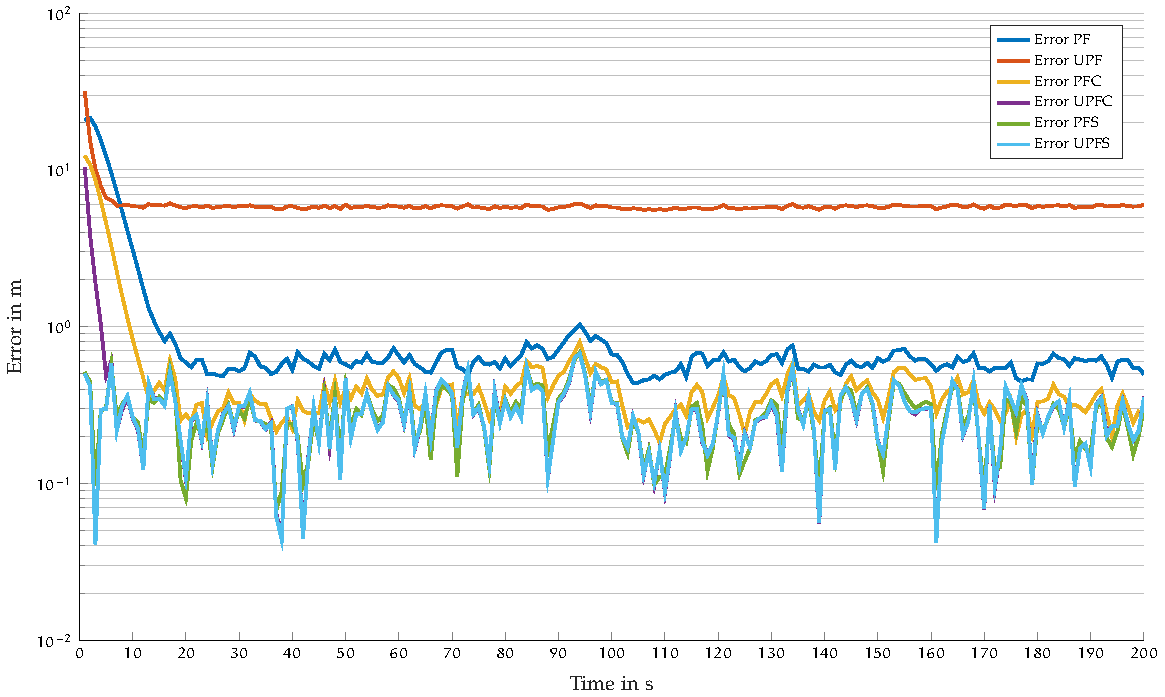
\includegraphics[height=1.0\textwidth]{Tikz/Results/2018-09-23-20-54-13-results-figure-5.tikz}}			
	\caption[Mean estimation error over time in Scenario 2. \texttt{PF}, \texttt{PFC}, \texttt{PFS}: 1000 particles. \texttt{UPF}, \texttt{UPFC}, \texttt{UPFS}: 10 particles.]{Mean estimation error over time in Scenario 2 (logarithmic scale). \texttt{PF}, \texttt{PFC}, \texttt{PFS}: 1000 particles. \texttt{UPF}, \texttt{UPFC}, \texttt{UPFS}: 10 particles.}
	\label{fig:2018-09-23-20-54-13-results-figure-5}			
\end{figure}

\begin{figure}
	\centering
	\setlength\figureheight{1.0\textwidth} 	
	\setlength\figurewidth{0.9\textheight}		
	\tikzsetnextfilename{2018-09-23-20-54-13-results-figure-7}		
	\rotatebox{90}{
	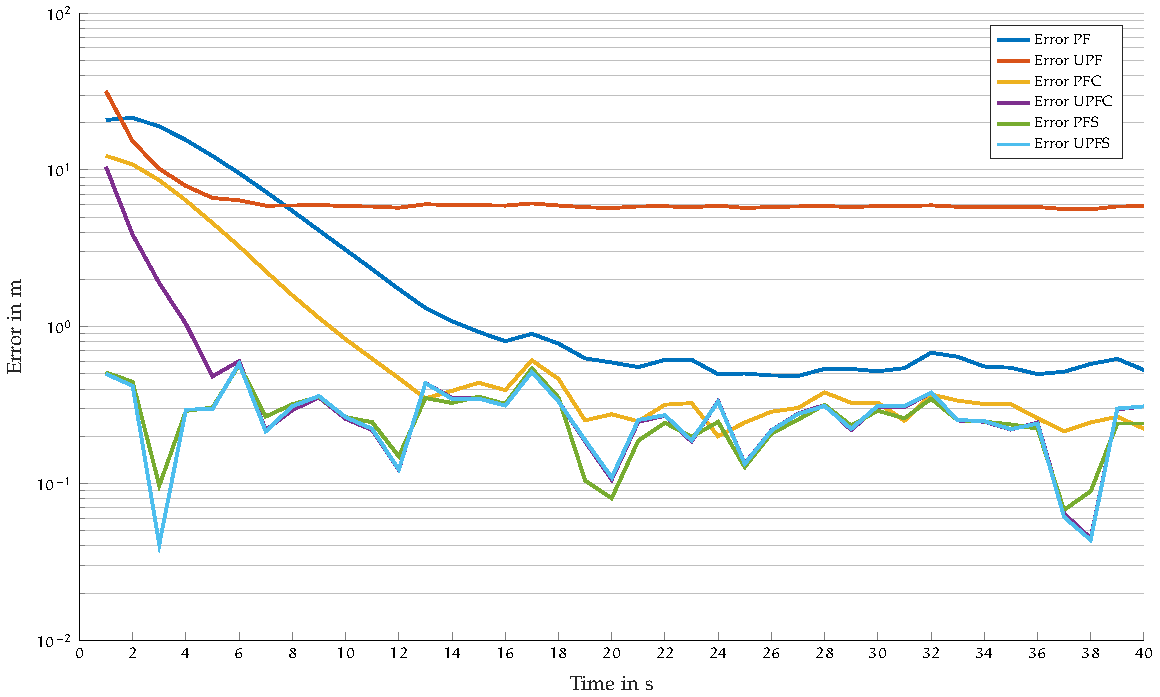
\includegraphics[height=1.0\textwidth]{Tikz/Results/2018-09-23-20-54-13-results-figure-7.tikz}}			
	\caption[First 40 seconds of the mean estimation error over time in Scenario 2. \texttt{PF}, \texttt{PFC}, \texttt{PFS}: 1000 particles. \texttt{UPF}, \texttt{UPFC}, \texttt{UPFS}: 10 particles.]{First 40 seconds of the mean estimation error over time in Scenario 2 (logarithmic scale). \texttt{PF}, \texttt{PFC}, \texttt{PFS}: 1000 particles. \texttt{UPF}, \texttt{UPFC}, \texttt{UPFS}: 10 particles.}
	\label{fig:2018-09-23-20-54-13-results-figure-7}			
\end{figure}


% 100 / 10

%\begin{figure}
%	\centering
%	\setlength\figureheight{0.9\textheight} 	
%	\setlength\figurewidth{1.0\textwidth}		
%	\tikzsetnextfilename{2018-09-21-16-00-07-results-figure-1}		
%	\includegraphics[width=\textwidth]{Tikz/Results/2018-09-21-16-00-07-results-figure-1.tikz}			
%	\caption[Box plot of the estimation errors in Scenario 2. \texttt{PF}, \texttt{PFC}, \texttt{PFS}: 100 particles. \texttt{UPF}, \texttt{UPFC}, \texttt{UPFS}: 10 particles.]{Box plot of the estimation errors in Scenario 2 (logarithmic scale). \texttt{PF}, \texttt{PFC}, \texttt{PFS}: 100 particles. \texttt{UPF}, \texttt{UPFC}, \texttt{UPFS}: 10 particles.}	
%	\label{fig:2018-09-21-16-00-07-results-figure-1}			
%\end{figure}
%
%\begin{figure}
%	\centering
%	\setlength\figureheight{1.0\textwidth} 	
%	\setlength\figurewidth{0.9\textheight}		
%	\tikzsetnextfilename{2018-09-21-16-00-07-results-figure-5}		
%	\rotatebox{90}{
%	\includegraphics[height=1.0\textwidth]{Tikz/Results/2018-09-21-16-00-07-results-figure-5.tikz}}			
%	\caption[Mean estimation error over time in Scenario 2. \texttt{PF}, \texttt{PFC}, \texttt{PFS}: 100 particles. \texttt{UPF}, \texttt{UPFC}, \texttt{UPFS}: 10 particles.]{Mean estimation error over time in Scenario 2 (logarithmic scale). \texttt{PF}, \texttt{PFC}, \texttt{PFS}: 100 particles. \texttt{UPF}, \texttt{UPFC}, \texttt{UPFS}: 10 particles.}
%	\label{fig:2018-09-21-16-00-07-results-figure-5}			
%\end{figure}
%
%\begin{figure}
%	\centering
%	\setlength\figureheight{1.0\textwidth} 	
%	\setlength\figurewidth{0.9\textheight}		
%	\tikzsetnextfilename{2018-09-21-16-00-07-results-figure-7}		
%	\rotatebox{90}{
%	\includegraphics[height=1.0\textwidth]{Tikz/Results/2018-09-21-16-00-07-results-figure-7.tikz}}			
%	\caption[First 40 seconds of the mean estimation error over time in Scenario 2. \texttt{PF}, \texttt{PFC}, \texttt{PFS}: 100 particles. \texttt{UPF}, \texttt{UPFC}, \texttt{UPFS}: 10 particles.]{First 40 seconds of the mean estimation error over time in Scenario 2 (logarithmic scale). \texttt{PF}, \texttt{PFC}, \texttt{PFS}: 100 particles. \texttt{UPF}, \texttt{UPFC}, \texttt{UPFS}: 10 particles.}
%	\label{fig:2018-09-21-16-00-07-results-figure-7}			
%\end{figure}

%% 4 Landmarks kidnapping


% 1000 / 10

\begin{figure}
	\centering
	\setlength\figureheight{0.9\textheight} 	
	\setlength\figurewidth{1.0\textwidth}		
	\tikzsetnextfilename{2018-09-23-12-42-11-results-figure-1}		
	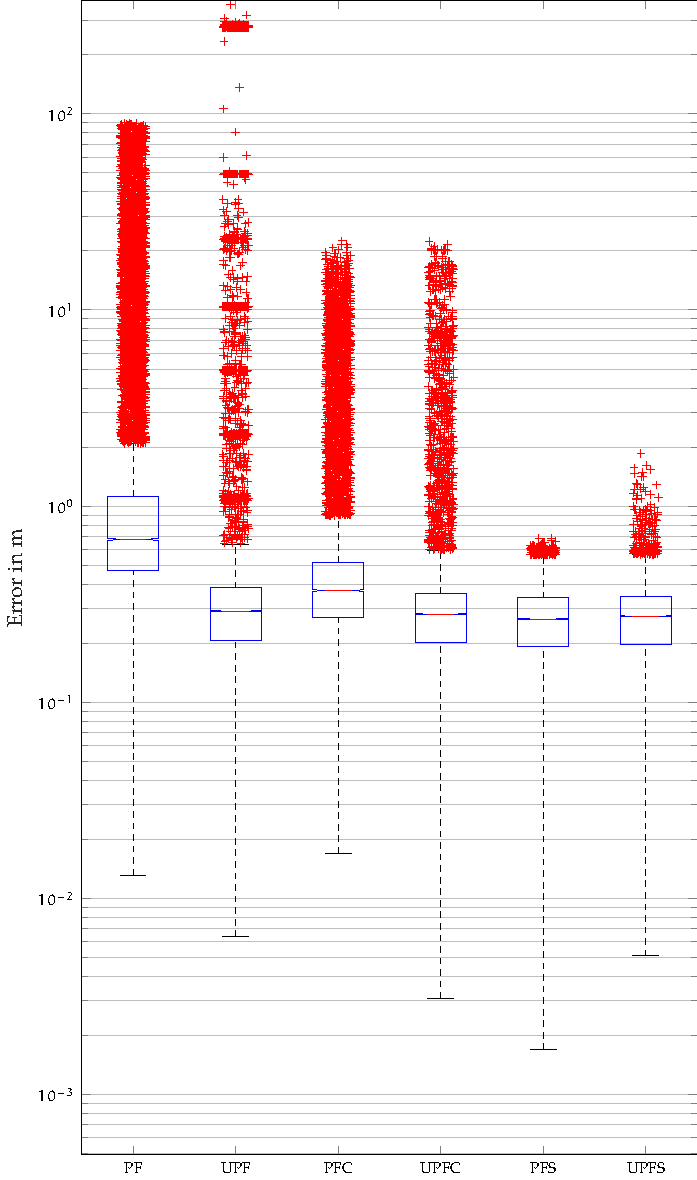
\includegraphics[width=\textwidth]{Tikz/Results/2018-09-23-12-42-11-results-figure-1.tikz}			
	\caption[Box plot of the estimation errors in Scenario 2 with kidnapping. \texttt{PF}, \texttt{PFC}, \texttt{PFS}: 1000 particles. \texttt{UPF}, \texttt{UPFC}, \texttt{UPFS}: 10 particles.]{Box plot of the estimation errors in Scenario 2 with kidnapping (logarithmic scale). \texttt{PF}, \texttt{PFC}, \texttt{PFS}: 1000 particles. \texttt{UPF}, \texttt{UPFC}, \texttt{UPFS}: 10 particles.}
	\label{fig:2018-09-23-12-42-11-results-figure-1}			
\end{figure}

\begin{figure}
	\centering
	\setlength\figureheight{1.0\textwidth} 	
	\setlength\figurewidth{0.9\textheight}		
	\tikzsetnextfilename{2018-09-23-12-42-11-results-figure-6}		
	\rotatebox{90}{
	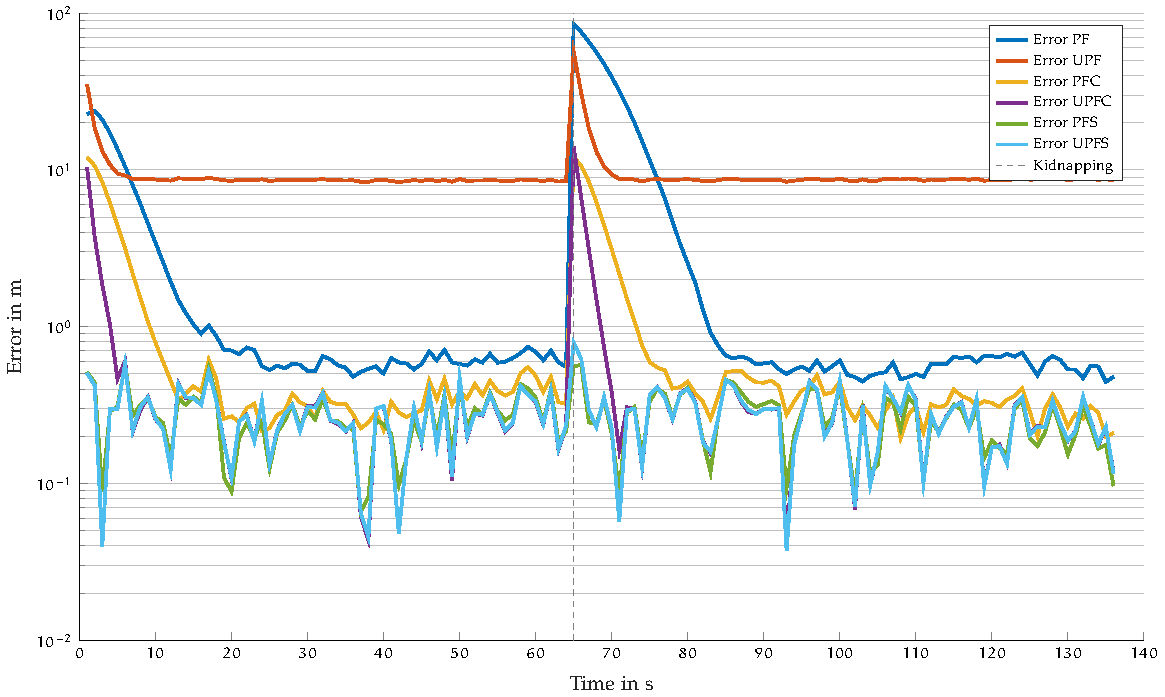
\includegraphics[height=1.0\textwidth]{Tikz/Results/2018-09-23-12-42-11-results-figure-6.tikz}}			
	\caption[Mean estimation error over time in Scenario 2 with kidnapping. \texttt{PF}, \texttt{PFC}, \texttt{PFS}: 1000 particles. \texttt{UPF}, \texttt{UPFC}, \texttt{UPFS}: 10 particles.]{Mean estimation error over time in Scenario 2 with kidnapping (logarithmic scale). \texttt{PF}, \texttt{PFC}, \texttt{PFS}: 1000 particles. \texttt{UPF}, \texttt{UPFC}, \texttt{UPFS}: 10 particles.}
	\label{fig:2018-09-23-12-42-11-results-figure-6}			
\end{figure}

\begin{figure}
	\centering
	\setlength\figureheight{1.0\textwidth} 	
	\setlength\figurewidth{0.9\textheight}		
	\tikzsetnextfilename{2018-09-23-12-42-11-results-figure-8}		
	\rotatebox{90}{
	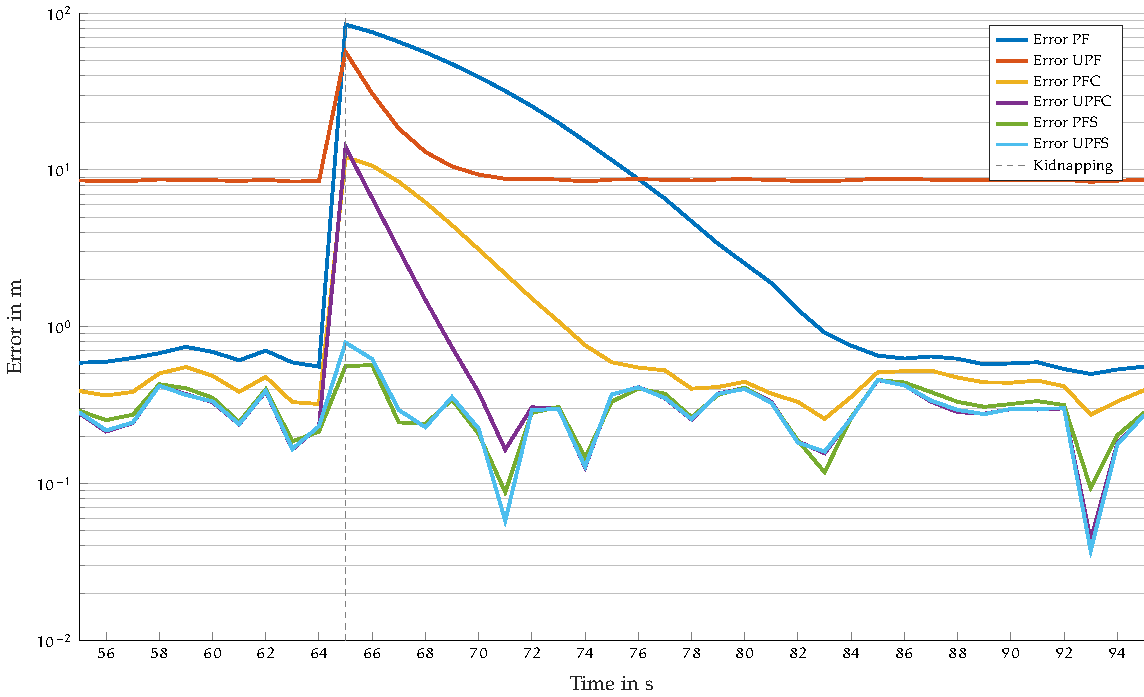
\includegraphics[height=1.0\textwidth]{Tikz/Results/2018-09-23-12-42-11-results-figure-8.tikz}}			
	\caption[First 30 seconds of the mean estimation error over time after kidnapping in Scenario 2. \texttt{PF}, \texttt{PFC}, \texttt{PFS}: 1000 particles. \texttt{UPF}, \texttt{UPFC}, \texttt{UPFS}: 10 particles.]{First 30 seconds of the mean estimation error over time after kidnapping in Scenario 2 (logarithmic scale). \texttt{PF}, \texttt{PFC}, \texttt{PFS}: 1000 particles. \texttt{UPF}, \texttt{UPFC}, \texttt{UPFS}: 10 particles.}	
	\label{fig:2018-09-23-12-42-11-results-figure-8}			
\end{figure}


% 100 / 10

%\begin{figure}
%	\centering
%	\setlength\figureheight{0.9\textheight} 	
%	\setlength\figurewidth{1.0\textwidth}		
%	\tikzsetnextfilename{2018-09-21-10-11-38-results-figure-1}		
%	\includegraphics[width=\textwidth]{Tikz/Results/2018-09-21-10-11-38-results-figure-1.tikz}			
%	\caption[Box plot of the estimation errors in Scenario 2 with kidnapping. \texttt{PF}, \texttt{PFC}, \texttt{PFS}: 100 particles. \texttt{UPF}, \texttt{UPFC}, \texttt{UPFS}: 10 particles.]{Box plot of the estimation errors in Scenario 2 with kidnapping (logarithmic scale). \texttt{PF}, \texttt{PFC}, \texttt{PFS}: 100 particles. \texttt{UPF}, \texttt{UPFC}, \texttt{UPFS}: 10 particles.}
%	\label{fig:2018-09-21-10-11-38-results-figure-1}			
%\end{figure}
%
%\begin{figure}
%	\centering
%	\setlength\figureheight{1.0\textwidth} 	
%	\setlength\figurewidth{0.9\textheight}		
%	\tikzsetnextfilename{2018-09-21-10-11-38-results-figure-6}		
%	\rotatebox{90}{
%	\includegraphics[height=1.0\textwidth]{Tikz/Results/2018-09-21-10-11-38-results-figure-6.tikz}}			
%	\caption[Mean estimation error over time in Scenario 2 with kidnapping. \texttt{PF}, \texttt{PFC}, \texttt{PFS}: 100 particles. \texttt{UPF}, \texttt{UPFC}, \texttt{UPFS}: 10 particles.]{Mean estimation error over time in Scenario 2 with kidnapping (logarithmic scale). \texttt{PF}, \texttt{PFC}, \texttt{PFS}: 100 particles. \texttt{UPF}, \texttt{UPFC}, \texttt{UPFS}: 10 particles.}
%	\label{fig:2018-09-21-10-11-38-results-figure-6}			
%\end{figure}
%
%\begin{figure}
%	\centering
%	\setlength\figureheight{1.0\textwidth} 	
%	\setlength\figurewidth{0.9\textheight}		
%	\tikzsetnextfilename{2018-09-21-10-11-38-results-figure-8}		
%	\rotatebox{90}{
%	\includegraphics[height=1.0\textwidth]{Tikz/Results/2018-09-21-10-11-38-results-figure-8.tikz}}			
%	\caption[First 30 seconds of the mean estimation error over time after kidnapping in Scenario 2. \texttt{PF}, \texttt{PFC}, \texttt{PFS}: 100 particles. \texttt{UPF}, \texttt{UPFC}, \texttt{UPFS}: 10 particles.]{First 30 seconds of the mean estimation error over time after kidnapping in Scenario 2 (logarithmic scale). \texttt{PF}, \texttt{PFC}, \texttt{PFS}: 100 particles. \texttt{UPF}, \texttt{UPFC}, \texttt{UPFS}: 10 particles.}	
%	\label{fig:2018-09-21-10-11-38-results-figure-8}			
%\end{figure}



%% 9 Landmarks

% 1000 / 10

\begin{figure}
	\centering
	\setlength\figureheight{0.9\textheight} 	
	\setlength\figurewidth{1.0\textwidth}		
	\tikzsetnextfilename{2018-09-01-16-39-24-results-figure-1}		
	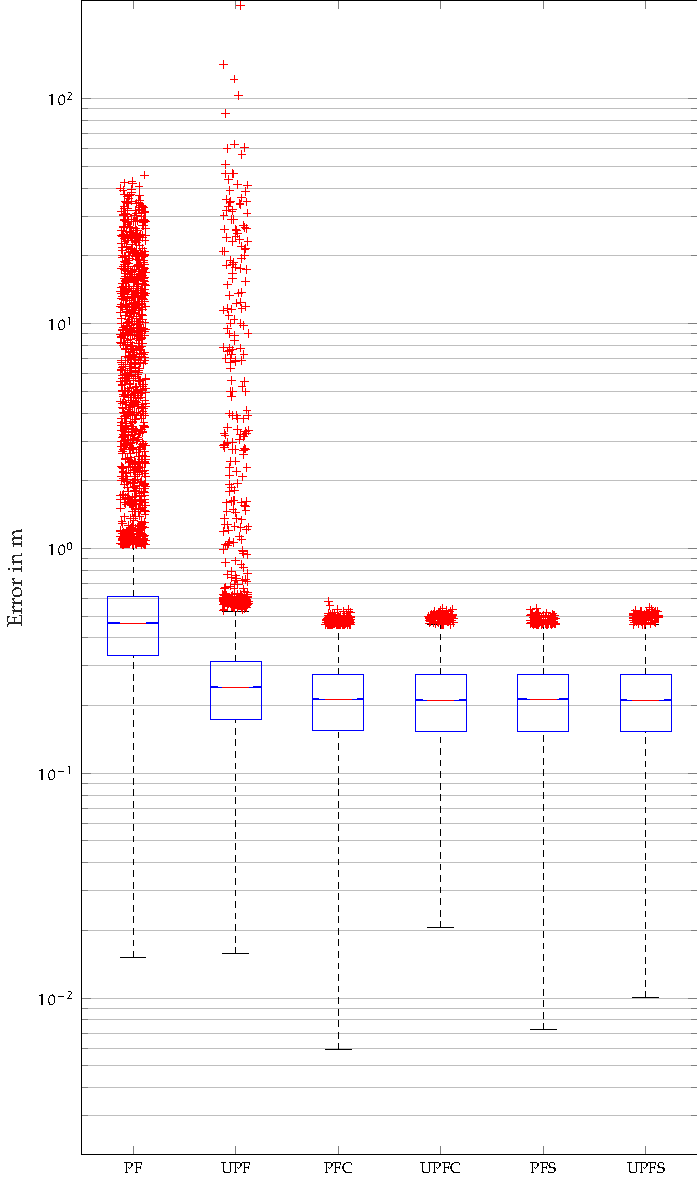
\includegraphics[width=\textwidth]{Tikz/Results/2018-09-01-16-39-24-results-figure-1.tikz}			
	\caption[Box plot of the estimation errors in Scenario 3. \texttt{PF}, \texttt{PFC}, \texttt{PFS}: 1000 particles. \texttt{UPF}, \texttt{UPFC}, \texttt{UPFS}: 10 particles.]{Box plot of the estimation errors in Scenario 3 (logarithmic scale). \texttt{PF}, \texttt{PFC}, \texttt{PFS}: 1000 particles. \texttt{UPF}, \texttt{UPFC}, \texttt{UPFS}: 10 particles.}
	\label{fig:2018-09-01-16-39-24-results-figure-1}			
\end{figure}

\begin{figure}
	\centering
	\setlength\figureheight{1.0\textwidth} 	
	\setlength\figurewidth{0.9\textheight}		
	\tikzsetnextfilename{2018-09-01-16-39-24-results-figure-4}		
	\rotatebox{90}{
	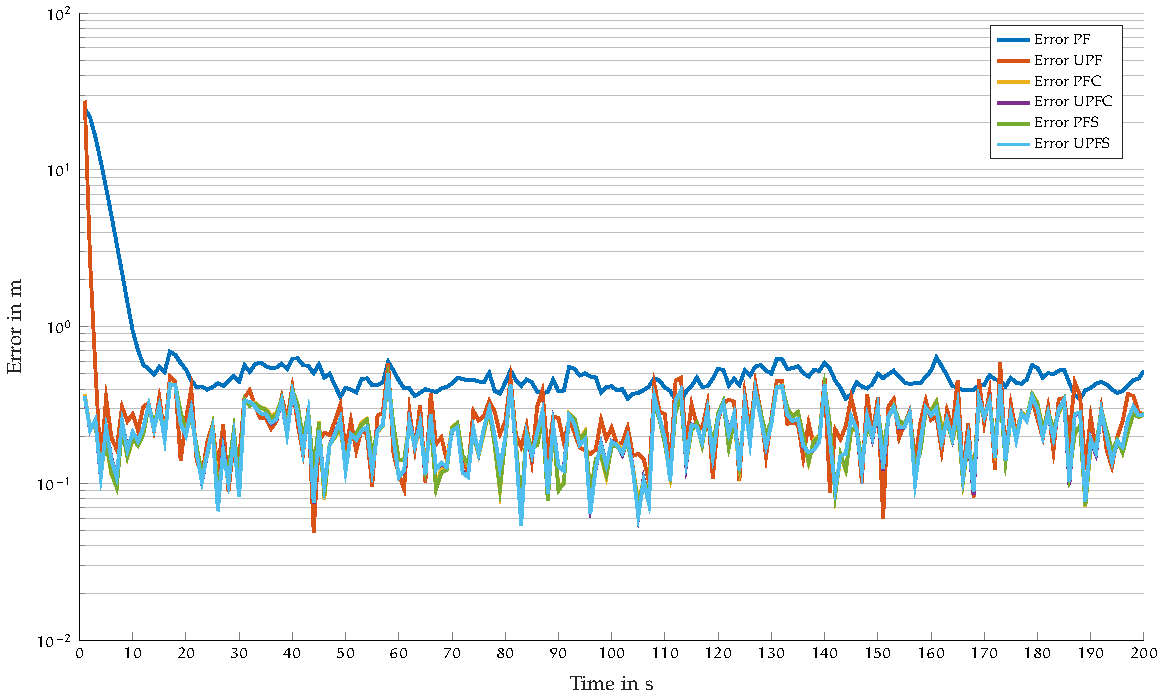
\includegraphics[height=1.0\textwidth]{Tikz/Results/2018-09-01-16-39-24-results-figure-4.tikz}}			
	\caption[Mean estimation error over time in Scenario 3. \texttt{PF}, \texttt{PFC}, \texttt{PFS}: 1000 particles. \texttt{UPF}, \texttt{UPFC}, \texttt{UPFS}: 10 particles.]{Mean estimation error over time in Scenario 3 (logarithmic scale). \texttt{PF}, \texttt{PFC}, \texttt{PFS}: 1000 particles. \texttt{UPF}, \texttt{UPFC}, \texttt{UPFS}: 10 particles.}
	\label{fig:2018-09-01-16-39-24-results-figure-4}			
\end{figure}

\begin{figure}
	\centering
	\setlength\figureheight{1.0\textwidth} 	
	\setlength\figurewidth{0.9\textheight}		
	\tikzsetnextfilename{2018-09-01-16-39-24-results-figure-6}		
	\rotatebox{90}{
	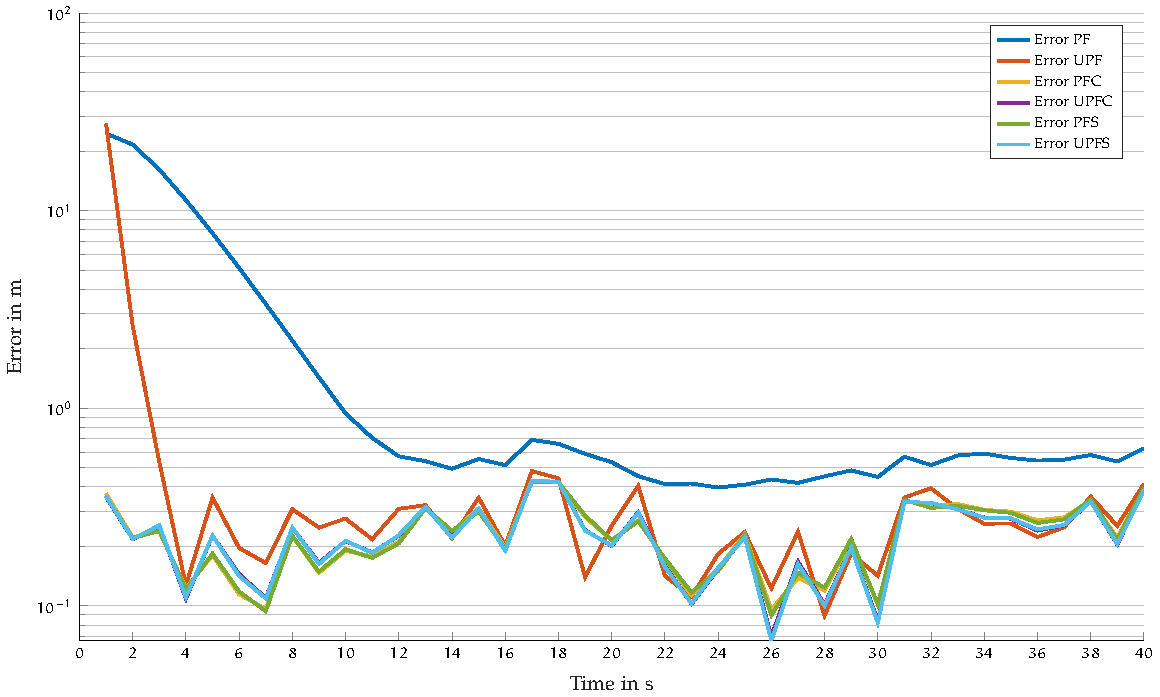
\includegraphics[height=1.0\textwidth]{Tikz/Results/2018-09-01-16-39-24-results-figure-6.tikz}}			
	\caption[First 40 seconds of the mean estimation error over time in Scenario 3. \texttt{PF}, \texttt{PFC}, \texttt{PFS}: 1000 particles. \texttt{UPF}, \texttt{UPFC}, \texttt{UPFS}: 10 particles.]{First 40 seconds of the mean estimation error over time in Scenario 3 (logarithmic scale). \texttt{PF}, \texttt{PFC}, \texttt{PFS}: 1000 particles. \texttt{UPF}, \texttt{UPFC}, \texttt{UPFS}: 10 particles.}
	\label{fig:2018-09-01-16-39-24-results-figure-6}			
\end{figure}


% 100 / 10

%\begin{figure}
%	\centering
%	\setlength\figureheight{0.9\textheight} 	
%	\setlength\figurewidth{1.0\textwidth}		
%	\tikzsetnextfilename{2018-09-02-11-42-39-results-figure-1}		
%	\includegraphics[width=\textwidth]{Tikz/Results/2018-09-02-11-42-39-results-figure-1.tikz}			
%	\caption[Box plot of the estimation errors in Scenario 3. \texttt{PF}, \texttt{PFC}, \texttt{PFS}: 100 particles. \texttt{UPF}, \texttt{UPFC}, \texttt{UPFS}: 10 particles.]{Box plot of the estimation errors in Scenario 3 (logarithmic scale). \texttt{PF}, \texttt{PFC}, \texttt{PFS}: 100 particles. \texttt{UPF}, \texttt{UPFC}, \texttt{UPFS}: 10 particles.}
%	\label{fig:2018-09-02-11-42-39-results-figure-1}			
%\end{figure}
%
%\begin{figure}
%	\centering
%	\setlength\figureheight{1.0\textwidth} 	
%	\setlength\figurewidth{0.9\textheight}		
%	\tikzsetnextfilename{2018-09-02-11-42-39-results-figure-4}		
%	\rotatebox{90}{
%	\includegraphics[height=1.0\textwidth]{Tikz/Results/2018-09-02-11-42-39-results-figure-4.tikz}}			
%	\caption[Mean estimation error over time in Scenario 3. \texttt{PF}, \texttt{PFC}, \texttt{PFS}: 100 particles. \texttt{UPF}, \texttt{UPFC}, \texttt{UPFS}: 10 particles.]{Mean estimation error over time in Scenario 3 (logarithmic scale). \texttt{PF}, \texttt{PFC}, \texttt{PFS}: 100 particles. \texttt{UPF}, \texttt{UPFC}, \texttt{UPFS}: 10 particles.}
%	\label{fig:2018-09-02-11-42-39-results-figure-4}			
%\end{figure}
%
%\begin{figure}
%	\centering
%	\setlength\figureheight{1.0\textwidth} 	
%	\setlength\figurewidth{0.9\textheight}		
%	\tikzsetnextfilename{2018-09-02-11-42-39-results-figure-6}		
%	\rotatebox{90}{
%	\includegraphics[height=1.0\textwidth]{Tikz/Results/2018-09-02-11-42-39-results-figure-6.tikz}}			
%	\caption[First 40 seconds of the mean estimation error over time in Scenario 3. \texttt{PF}, \texttt{PFC}, \texttt{PFS}: 100 particles. \texttt{UPF}, \texttt{UPFC}, \texttt{UPFS}: 10 particles.]
%	{First 40 seconds of the mean estimation error over time in Scenario 3 (logarithmic scale). \texttt{PF}, \texttt{PFC}, \texttt{PFS}: 100 particles. \texttt{UPF}, \texttt{UPFC}, \texttt{UPFS}: 10 particles.}
%	\label{fig:2018-09-02-11-42-39-results-figure-6}			
%\end{figure}


%% 9 Landmarks kidnapping

% 1000 / 10

\begin{figure}
	\centering
	\setlength\figureheight{0.9\textheight} 	
	\setlength\figurewidth{1.0\textwidth}		
	\tikzsetnextfilename{2018-09-07-08-54-39-results-figure-1}		
	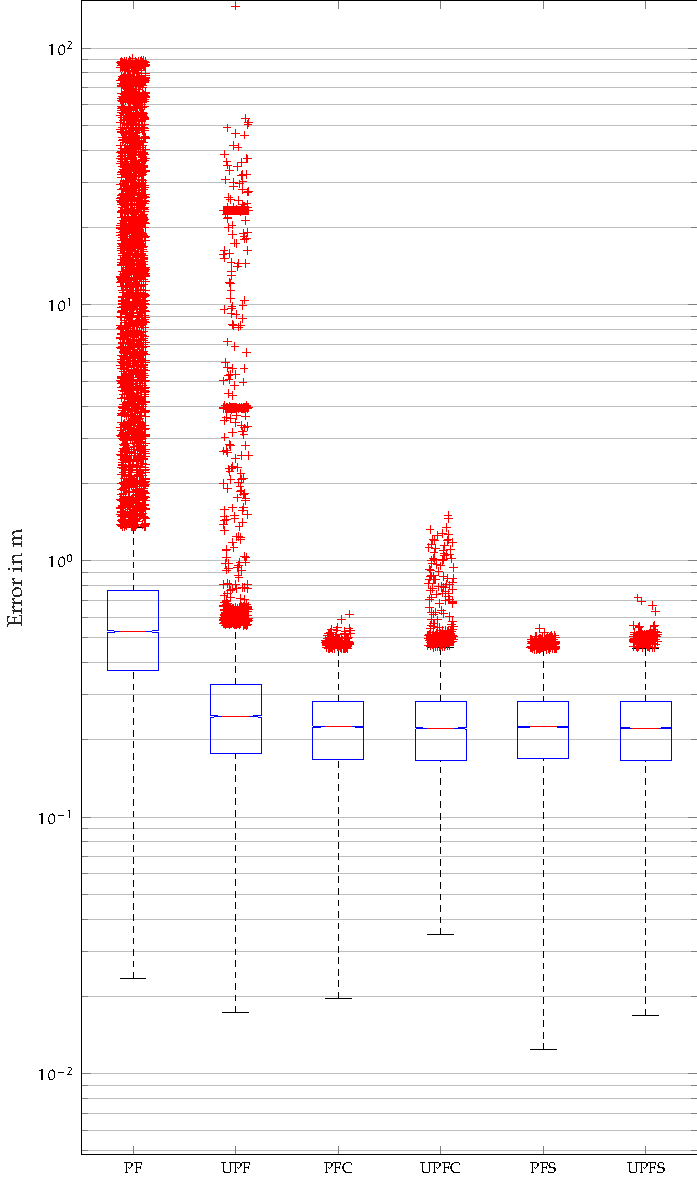
\includegraphics[width=\textwidth]{Tikz/Results/2018-09-07-08-54-39-results-figure-1.tikz}			
	\caption[Box plot of the estimation errors in Scenario 3 with kidnapping. \texttt{PF}, \texttt{PFC}, \texttt{PFS}: 1000 particles. \texttt{UPF}, \texttt{UPFC}, \texttt{UPFS}: 10 particles.]{Box plot of the estimation errors in Scenario 3 with kidnapping (logarithmic scale). \texttt{PF}, \texttt{PFC}, \texttt{PFS}: 1000 particles. \texttt{UPF}, \texttt{UPFC}, \texttt{UPFS}: 10 particles.}		
	\label{fig:2018-09-07-08-54-39-results-figure-1}			
\end{figure}

\begin{figure}
	\centering
	\setlength\figureheight{1.0\textwidth} 	
	\setlength\figurewidth{0.9\textheight}		
	\tikzsetnextfilename{2018-09-07-08-54-39-results-figure-4}		
	\rotatebox{90}{
	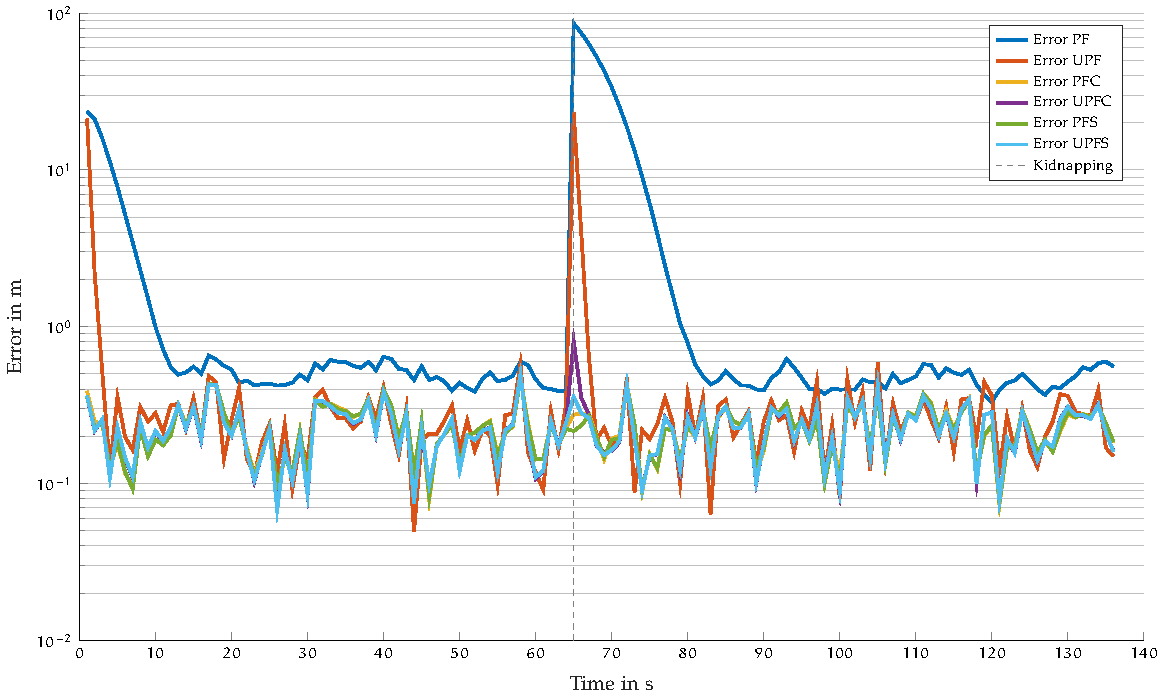
\includegraphics[height=1.0\textwidth]{Tikz/Results/2018-09-07-08-54-39-results-figure-4.tikz}}			
	\caption[Mean estimation error over time in Scenario 3 with kidnapping. \texttt{PF}, \texttt{PFC}, \texttt{PFS}: 1000 particles. \texttt{UPF}, \texttt{UPFC}, \texttt{UPFS}: 10 particles.]{Mean estimation error over time in Scenario 3 with kidnapping (logarithmic scale). \texttt{PF}, \texttt{PFC}, \texttt{PFS}: 1000 particles. \texttt{UPF}, \texttt{UPFC}, \texttt{UPFS}: 10 particles.}
	\label{fig:2018-09-07-08-54-39-results-figure-4}			
\end{figure}

\begin{figure}
	\centering
	\setlength\figureheight{1.0\textwidth} 	
	\setlength\figurewidth{0.9\textheight}		
	\tikzsetnextfilename{2018-09-07-08-54-39-results-figure-6}
	\rotatebox{90}{
	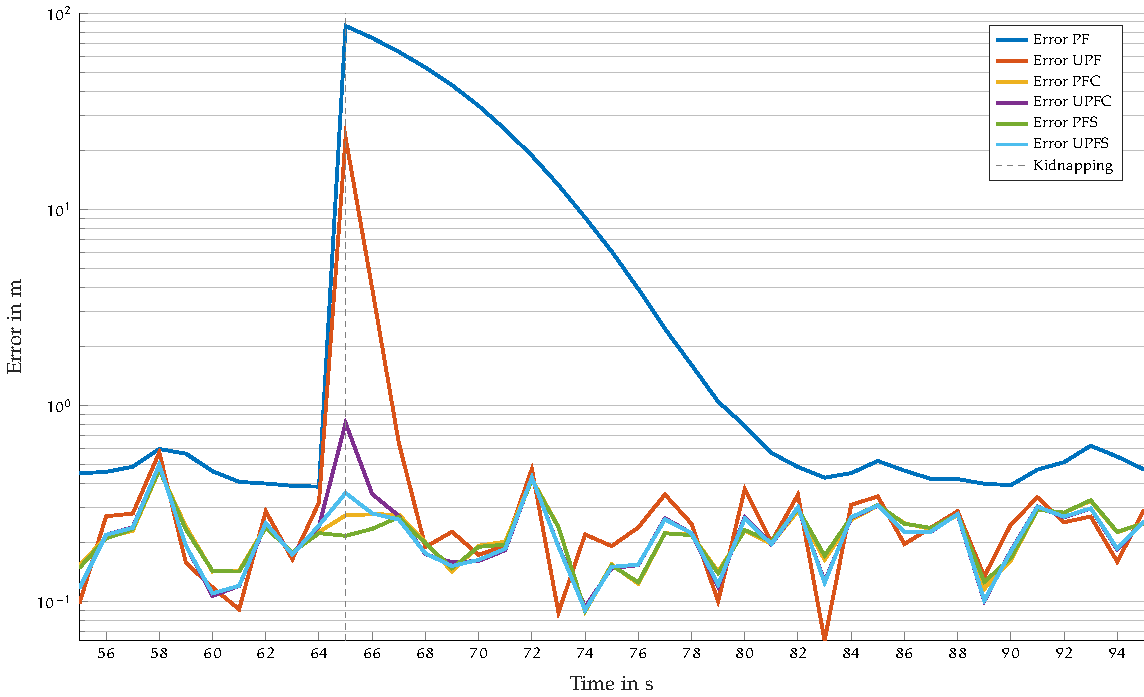
\includegraphics[height=1.0\textwidth]{Tikz/Results/2018-09-07-08-54-39-results-figure-6.tikz}}			
	\caption[First 30 seconds of the mean estimation error over time after kidnapping in Scenario 3. \texttt{PF}, \texttt{PFC}, \texttt{PFS}: 1000 particles. \texttt{UPF}, \texttt{UPFC}, \texttt{UPFS}: 10 particles.]{First 30 seconds of the mean estimation error over time after kidnapping in Scenario 3 (logarithmic scale). \texttt{PF}, \texttt{PFC}, \texttt{PFS}: 1000 particles. \texttt{UPF}, \texttt{UPFC}, \texttt{UPFS}: 10 particles.}
	\label{fig:2018-09-07-08-54-39-results-figure-6}			
\end{figure}


% 100 / 10

%\begin{figure}
%	\centering
%	\setlength\figureheight{0.9\textheight} 	
%	\setlength\figurewidth{1.0\textwidth}		
%	\tikzsetnextfilename{2018-09-18-11-37-10-results-figure-1}
%	\includegraphics[width=\textwidth]{Tikz/Results/2018-09-18-11-37-10-results-figure-1.tikz}			
%	\caption[Box plot of the estimation errors in Scenario 3 with kidnapping. \texttt{PF}, \texttt{PFC}, \texttt{PFS}: 100 particles. \texttt{UPF}, \texttt{UPFC}, \texttt{UPFS}: 10 particles.]{Box plot of the estimation errors in Scenario 3 with kidnapping (logarithmic scale). \texttt{PF}, \texttt{PFC}, \texttt{PFS}: 100 particles. \texttt{UPF}, \texttt{UPFC}, \texttt{UPFS}: 10 particles.}		
%	\label{fig:2018-09-18-11-37-10-results-figure-1}			
%\end{figure}
%
%\begin{figure}
%	\centering
%	\setlength\figureheight{1.0\textwidth} 	
%	\setlength\figurewidth{0.9\textheight}		
%	\tikzsetnextfilename{2018-09-18-11-37-10-results-figure-5}		
%	\rotatebox{90}{
%	\includegraphics[height=1.0\textwidth]{Tikz/Results/2018-09-18-11-37-10-results-figure-5.tikz}}			
%	\caption[Mean estimation error over time in Scenario 3 with kidnapping. \texttt{PF}, \texttt{PFC}, \texttt{PFS}: 100 particles. \texttt{UPF}, \texttt{UPFC}, \texttt{UPFS}: 10 particles.]{Mean estimation error over time in Scenario 3 with kidnapping (logarithmic scale). \texttt{PF}, \texttt{PFC}, \texttt{PFS}: 100 particles. \texttt{UPF}, \texttt{UPFC}, \texttt{UPFS}: 10 particles.}
%	\label{fig:2018-09-18-11-37-10-results-figure-5}			
%\end{figure}
%
%\begin{figure}
%	\centering
%	\setlength\figureheight{1.0\textwidth} 	
%	\setlength\figurewidth{0.9\textheight}		
%	\tikzsetnextfilename{2018-09-18-11-37-10-results-figure-7}		
%	\rotatebox{90}{
%	\includegraphics[height=1.0\textwidth]{Tikz/Results/2018-09-18-11-37-10-results-figure-7.tikz}}			
%	\caption[First 30 seconds of the mean estimation error over time after kidnapping in Scenario 3. \texttt{PF}, \texttt{PFC}, \texttt{PFS}: 100 particles. \texttt{UPF}, \texttt{UPFC}, \texttt{UPFS}: 10 particles.]{First 30 seconds of the mean estimation error over time after kidnapping in Scenario 3 (logarithmic scale). \texttt{PF}, \texttt{PFC}, \texttt{PFS}: 100 particles. \texttt{UPF}, \texttt{UPFC}, \texttt{UPFS}: 10 particles.}	\label{fig:2018-09-18-11-37-10-results-figure-7}
%\end{figure}




